\documentclass{article}

\usepackage{graphicx}
\usepackage{amsmath}
\usepackage{mathtools}

\usepackage[utf8]{inputenc}
\usepackage[english]{babel}
\usepackage{mathrsfs,amsmath}
\usepackage{float}
\usepackage{subfig}


% Puts captions of tables on top
\floatstyle{plaintop}
\restylefloat{table}

% Puts captions in bold
\captionsetup{labelfont=bf}

\begin{document}

\begin{titlepage}
\begin{center}

\textsc{\LARGE Delft University of Technology}\\[1.5cm]
\textsc{ SC4045 Control for High Resolution Imaging}\\[0.5cm]

% Title
{\huge\bfseries Wavefront Reconstruction \\[0.4cm] }

% Author and supervisor
\begin{minipage}{0.4\textwidth}
\begin{flushleft} \large
\emph{Author:}\\
Jacco v.d. Spek \\
4002512 \\
Niels Tielen \\
4011147

\end{flushleft}
\end{minipage}
\begin{minipage}{0.4\textwidth}
\begin{flushright} \large
\emph{Supervisors:} \\
Prof. M. Verhaegen \\
João P. Lopes e Silva  
\end{flushright}
\end{minipage}

\vfill
% Bottom of the page
{\large \today}
\end{center}
\end{titlepage}

\section*{Introduction}

In the previous part of this report, we already mentioned the first steps in the use of adaptive optics. First we described wavefront generating and wavefront sensing. In this chapter of the report, we direct our focus to the reconstruction of the wavefront. 

\section{Zonal Reconstruction}
In order to describe the gradient of the wavefront, we first take a look at a zonal reconstruction method. With zonal reconstruction, we split up the wavefront in zones. These zones can represent a regular grid of square or rectangular elements or some other local region such as a hexagon or other shape. For Shack-Hartmann wavefront sensors, the type of sensor that is used, these zones are generally chosen to match the lenslet array.

\subsection{reconstruction of wavefront slopes}
As can be seen in the part of the centroid algorithm, the relation between the slope of the wavefront and the wavefront phase can be defined by the following partial derivative:
$$ \sigma_x = \frac{\partial\phi(x,y)}{\partial x},$$ 
$$ \sigma_y = \frac{\partial\phi(x,y)}{\partial y}.$$ 
Where $\sigma_x$ and $\sigma_y$ approximate the gradient of the phase in the $x$ and $y$ direction, respectively.
In order to estimate the derivatives, we need to use a finite difference (FD) method. There are a number of different FD methods which depend on the sampling geometry. Some of these geometries are the Fried~\cite{fried1977least}, Hudgin~\cite{hudgin1977wave} and Southwell~\cite{southwell1980wave} geometries. We first start with a detailed explanation of the Fried geometry.

\subsection{Fried Geometry}
The Fried FD method calculates the average slope in one grid cell by using the four phase points. We first take a look at one part of the cell grid.
\begin{figure}[h!]
  \centering
  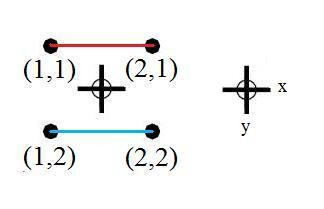
\includegraphics[scale=0.6]{figures/fried}
  \caption{slope approximation, Fried}
\end{figure}
\newpage
\noindent The goal is to calculate average of the both slopes. The first slope (in the x-direction) is given by the red line. We can easily see that this slope is given by:
$$ \sigma_{x,\text{red}} = \frac{\phi(2,1) - \phi(1,1)}{h}, $$
where $h$ is the step between the 2 phase measurements, usually the size of the subaperture.

Now we do the same for the other slope:
$$ \sigma_{x,\text{blue}} = \frac{\phi(2,2) - \phi(1,2)}{h}. $$
Now we take the average of these 2 slopes on then we know the slope of the wavefront in this zone (for x-direction).
$$ \sigma_x = \frac{\sigma_{x,\text{red}}+\sigma_{x,\text{blue}}}{2}$$
And when substituted:
$$ \sigma_x = \frac{(\phi(2,1) - \phi(1,1))+(\phi(2,2) - \phi(1,2))}{2h}$$
From this example, we can derive a general method for calculating the slope. 
$$ \sigma_x = \frac{[(\phi(i+1,j)-\phi(i,j))+(\phi(i+1,j+1)-\phi(i,j+1)]}{2h} + n_x(i,j)$$
$$ \sigma_y = \frac{[(\phi(i,j+1)-\phi(i,j))+(\phi(i+1,j+1)-\phi(i+1,j)]}{2h} + n_y(i,j)$$
We also add noise, to introduce the effect of measurement error and approximation errors.
This is the Fried geometry model. Later in this chapter the Southwell and Hudgin geometries will be introduced, but for now we will consider the Fried FD model as the default geometry.

\subsection{Creating the geometry matrix}
The next step is to take geometry model and structurize it in an orderly fashion. We structurize the model as followed:
$$ s = G\phi + n.$$  
Here s is the vector containing the slopes, made by appending $[\sigma_x^top \sigma_y^top]^\top$. The symbol $\phi$ is a vector filled with the phase points used define the slope and n is the noise. The equations used to link $\phi$ with $s$ can be found in the geometry matrix G. In our previous example we can derive the following G matrix:
$$ 
\begin{bmatrix}
\sigma_x \\
\sigma_y
\end{bmatrix} 
=
G
\cdot
\begin{bmatrix}
\phi(1,1) \\
\phi(2,1) \\
\phi(1,2) \\
\phi(2,2) 
\end{bmatrix}
$$
Where, in this case, G is defined as:
$$
G
=
\frac{\alpha}{2h}
\begin{bmatrix}
-1 & 1 & -1 & 1 \\
-1 & -1 & 1 & 1 \\
\end{bmatrix}
$$

\subsection{Hudgin Geometries}
As mentioned before, there are many other geometries that can be used to generate a geometry matrix. Earlier we mentioned the Hudgin an Southwell geometry besides the Fried geometry. We first start to take a closer look at the Hudgin geometry.
\newline
\newline
Lets take a look at the way the Hudgin geometry is defined. First we start with an overview of the slopes and phase points.
\begin{figure}[h!]
  \centering
  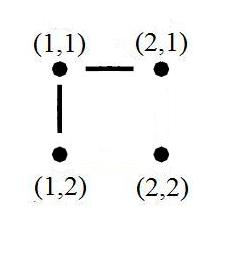
\includegraphics[scale=0.6]{figures/hudgin}
  \caption{slope approximation, Hudgin}
\end{figure}
From this we can easily derive the slope approximation in x and y direction. These are given by the following equations:
$$ \sigma_x = \frac{\phi(2,1)-\phi(1,1)}{h}$$
$$ \sigma_x = \frac{\phi(1,2)-\phi(1,1)}{h}$$
From these equations we can derive the geometry matrix, just as we have done with the Fried geometry. But if we look closer to Figure 2, we see that slopes $\sigma_x$ and $\sigma_y$ are not defined in the same point, as with the Fried geometry. Due to our sensor, the Shack-Hartmann sensor, and it`s centroid algorithm, we only the 2 slopes in the same point. As this geometry requires the slopes at 2 different pionts, we have to conclude that we cannot use the Hudgin geometry. But fortunately, we can alter the Hudgin geometry slightly, and use it on a Shack-Hartmann sensor. This is called the `Modified` Hudgin geometry\cite{rosensteiner2011cumulative}.

\newline
\newline
The Modified Hudgin geometry uses the same theory as the Hudgin geometry, but it makes it capable for being used in a Shack-Hartmann sensor. Let`s see an overview of the slopes and phase points as they are used in the Modified Hudgin geometry.  

\begin{figure}[h!]
  \centering
  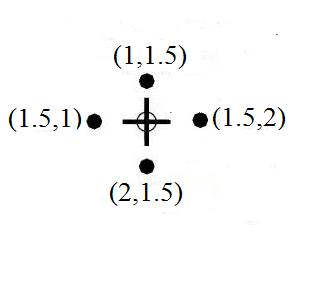
\includegraphics[scale=0.6]{figures/mod_hudgin}
  \caption{slope approximation, Modified Hudgin}
\end{figure}
\noindent Now it is clear to see that we can use the slope information from the centroid algorithm to define four phase points to do the reconstruction. Now we can derive the equations that define the 2 slopes:
$$ \sigma_x = \frac{\phi(2,1.5)-\phi(1,1.5)}{h}$$
$$ \sigma_y = \frac{\phi(1.5,2)-\phi(1.5,1)}{h}$$
And just as we did with the Fried geometry, we can define a geometry matrix~$G$:
$$ 
\begin{bmatrix}
\sigma_x \\
\sigma_y
\end{bmatrix} 
=
G
\cdot
\begin{bmatrix}
\phi(1,1.5) \\
\phi(1.5,1) \\
\phi(1.5,2) \\
\phi(2,1.5) 
\end{bmatrix}
$$
Where, in this case, G is defined as:
$$
G
=
\frac{\alpha}{h}
\begin{bmatrix}
0 & -1 & 1 & 0 \\
-1 & 0 & 0 & 1 \\
\end{bmatrix}
$$


\subsection{Southwell Geometries}
The last geometry which will be examined is the Southwell geometry. In the case of Southwell geometry, the phase points lie in the same place as the points where the slopes are defined. If we take a look at an overview where these points are defined, we can then define a relationship between the phase points and the slopes.


\begin{figure}[h!]
  \centering
  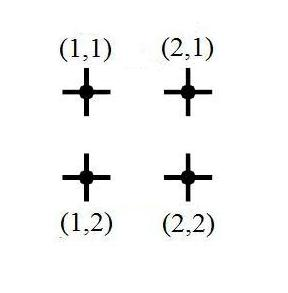
\includegraphics[scale=0.6]{figures/southwell}
  \caption{slope approximation, Southwell}
\end{figure}
\noindent From our first look at the overview, we can see slopes are placed exactly the same as with the Fried and Modified Hudgin geometries. This means that we can use Southwell geometry in our Shack-Hartmann sensor. 
\newline
\newline
Now it is time to look at how we define the relation between the slopes and the phase points. 
$$ \frac{\sigma_x(2,1)-\sigma_x(1,1)}{2} = \frac{\phi(2,1)-\phi(1,1)}{h}$$
$$ \frac{\sigma_y(1,2)-\sigma_y(1,1)}{2} = \frac{\phi(1,2)-\phi(1,1)}{h}$$
We can see that this geometry takes the average of the two slopes, in x and y-direction, and uses that to approximate the phase points. For our simple 2x2 example, we can add the following equations:
$$ \frac{\sigma_x(2,2)-\sigma_x(1,2)}{2} = \frac{\phi(2,2)-\phi(1,2)}{h}$$
$$ \frac{\sigma_y(2,2)-\sigma_y(2,1)}{2} = \frac{\phi(2,2)-\phi(2,1)}{h}$$
Again, we can rewrite this set of equations in a matrix, where we can define a geometry matrix. 
Unfortunately, due to the nature of the equations posted above, it is not that straightforward to define the geometry matrix. For this geometry we need to take another step. We first start to add a dummy variable $\varSigma$ to the equations above. We means we get:
$$ \frac{\sigma_x(2,1)-\sigma_x(1,1)}{2} = \frac{\phi(2,1)-\phi(1,1)}{h} = \varSigma_{x1}$$
$$ \frac{\sigma_x(2,2)-\sigma_x(1,2)}{2} = \frac{\phi(2,2)-\phi(1,2)}{h} = \varSigma_{x2}$$
$$ \frac{\sigma_y(1,2)-\sigma_y(1,1)}{2} = \frac{\phi(1,2)-\phi(1,1)}{h} = \varSigma_{y1}$$
$$ \frac{\sigma_y(2,2)-\sigma_y(2,1)}{2} = \frac{\phi(2,2)-\phi(2,1)}{h} = \varSigma_{y2}$$

Now we break this equation in two parts, for both the slopes and the phase points.
$$ \varSigma = AS$$
and
$$ \varSigma = B\phi$$ 
Which we can substitute:
$$ AS = B\phi $$
and get the geometry matrix which maps S and $\phi$:
$$ S = A^{-1}B\phi $$
In our simple 2x2 case, we can define the following A and B matrices:
\newline
\newline
$ A=
\begin{bmatrix}
-1 & 1 & 0 & 0 & 0 & 0 & 0 & 0  \\
 0 & 0 & -1& 1 & 0 & 0 & 0 & 0  \\
 0 & 0 & 0 & 0 & -1& 1 & 0 & 0  \\
 0 & 0 & 0 & 0 & 0 & 0 & -1& 1  \\
\end{bmatrix}
$
$
B = 
\begin{bmatrix}
-1 & 1 & 0 & 0 \\
 0 & 0 & -1& 1 \\
-1 & 0 & 1 & 0 \\
 0 & -1& 0 & 1 \\
\end{bmatrix}
$
\newline
\newline
And this leads to the following G:
$$
G = A^{-1}B 
$$

\newpage
\subsection{Least squares estimations}
No matter what geometry we choose, we always can write our reconstruction problem as followed:
$$ S=G\phi +n$$
As we have a overdefined set of equations, we need to estimate the solution to this problem. For this, we can use the least squares estimation. We are first going to look at a regular least squares problem
\newline
\newline
We first start with inconsistent set of equations:
$$ y=Fx $$
We would like to find the optimal solution $\hat{x}$, which we can write as:
\newline
\newline
\begin{equation*}
\begin{aligned}
& \underset{x}{\text{minimize}}
& & \epsilon^T\epsilon \\
& \text{subject to}
& & y=Fx + \epsilon
\end{aligned}
\end{equation*}
\newline
\newline
Where $\epsilon$ is the residual vector. We can rewrite the equation above in a more standard problem:
$$ min_x\|Fx-y\|_2^2$$ 
After expanding the above expression, computing the gradient and setting the gradient to 0, we derive the following equation:
$$ F^TF\hat{x}=F^Ty $$
which gives us the least squares estimator $\hat{x}$
$$ \hat{x} = (F^TF)^{-1}F^Ty $$
In this case, the matrix $(F^TF)^{-1}F^T$ is called a pseudo inverse, namely the Moore-Penrose inverse.
When using this estimator, the reconstruction problem can be solved by:
$$ \hat{\phi} = (G^TG)^{-1}G^TS  $$
\newline
\newline

Unfortunatly, our problem is defined slightly different. We need to think about the fact that we also have noise in our equations, which means that we cannot take $\phi$ as a determinstic vector. Note that we have noise info and `a priori` information about the phase available. In that case, we need to formulate the stochastic least squares problem. We would like to minimize the following equation:
$$ y=Fx+L\epsilon$$
From which we know that x has a mean of $\bar{x}$ and the covariance matrix P, which we consider to be positive-definite.
$\epsilon$ is consider white and is not correlated to x. We know that the solution to this problem has to be unbiased and have a minimum-variance. We first specify our linear estimator as:
$$ \tilde{x} = 
\begin{bmatrix}
M & N \\
\end{bmatrix}
\begin{bmatrix}
y \\
\bar{x}
\end{bmatrix}
$$
We first start from the fact that the solution must be unbiased. This means that the following must hold.
$$ E[\tilde{x}]=MF\bar{x} + N\bar{x}=(MF+N)\bar{x}$$
Which means:
$$MF+N=I$$  
Now we are going to look at the variance:
$$x-\tilde{x}=(I-MF)(x-\tilde{x})-ML\epsilon$$
And the expected value:
$$ E[(x-\tilde{x})(x-\tilde{x})^T] = (I-MF)P(I-MF)^T - M(LL^T)M^T$$
This equations can be expended to:
$$ E[(x-\tilde{x})(x-\tilde{x})^T] =
\begin{bmatrix}
I & -M \\
\end{bmatrix}
\begin{bmatrix}
P  & PF^T \\
FP & FPF^T+(LL^T)
\end{bmatrix}
\begin{bmatrix}
I  \\
-m^T
\end{bmatrix}
$$ 
Now the middle of this matrices can be expanded by using the Schur complement and next substituted back into the equation. After completing the squares, we can derive the matrix M that mimimizes the variance.
$$ M = PF^T(FPF^T+(LL^T))^{-1}$$
Which gives the solution to the stochastic least squares problem.
$$\tilde{x} = PF^T(FPF^T+(LL^T))^{-1}y$$
Now we have a the tools to solve our reconstruction problem.
\newline
\newline
$ min_x \ \ \epsilon^T \epsilon $, subjected to $ s=G\phi + L\epsilon$
\newline
\newline
where $E[\phi\phi^T]=C_\phi$ and $LL^T=C_n$. The solution is given by:
$$\hat{\phi} = C_\phi G^T(GC_\phi G^T + C_n)^{-1}S $$

\newpage
\section{Modal reconstruction}
In the previous chapter we have tried to reconstruct the wavefront using the zonal approach. Now we view another technique, the modal wavefront reconstruction. In modal reconstruction, we use a linear combination of basis polynomials over the entire aperture. These basis polynomials can be Zernike polynomials, Karhunen-Loeve functions, Legendre polynomials and Fourier series. In this report we will stick to the use of Zernike polynomials, as they are also used in the wavefront generation part. 

\subsection{Zernike polynomials}
In the case of modal reconstruction, we can express the wavefront as followed:
$$
\phi (x,y) = \sum_{k=0}^{M}a_kZ_k(x,y), 
$$
Where $a_k$ is the coefficient that needs to be calculated and $Z_k$ is the basis polynomial, in our case the Zernike polynomial. The Zernike polynomial is defined as followed:
$$
Z_u^v(\rho,\theta) = \sqrt{\frac{2(u+1)}{1+\delta(v,0)}}\sum_{s=0}^{\frac{u-v}{2}}\frac{(-1)^s(u-s)!}{s!(\frac{u+v}{2}-s)!(\frac{u-v}{2}-s)!}
\rho^{u-2s}cos(v\theta),
$$
with $\delta(v,0)$ the Kronecker Delta that is equal to 1 if v = 0 and zero otherwise. In the definition above, we used polar notation but with a slight abuse of notation, we can represent the wavefront as:
$$
\phi (x,y,\xi) = \sum_{u=0}^{u_{max}}\sum_{v=0}^{v_{max}}z_{uv}Z_u^v(x,y),
$$
with $\xi$ the vector containing all the coefficients $z_{uv}$.
Now we can represent the wavefront in terms of a polynomial, but the only information that is given by the wavefront sensor is the slope. Therefore we need to take a look at the spatial derivatives of the Zernike polynomials:
$$
\frac{\partial \phi(x,y)}{\partial x} = \sum_{u,v}z_{u,v}\frac{\partial Z_u^v(x,y)}{\partial x},
$$
$$
\frac{\partial \phi(x,y)}{\partial y} = \sum_{u,v}z_{u,v}\frac{\partial Z_u^v(x,y)}{\partial y}.
$$
Again, we can write this set of equations more effectively into the following matrix notation:
$$
\begin{bmatrix}
\sigma_x(i,j) \\
\sigma_y(i,j)
\end{bmatrix}
=
\begin{bmatrix}
\sum_{u,v}z_{u,v}\frac{\partial Z_u^v(x,y)}{\partial x} \\
\sum_{u,v}z_{u,v}\frac{\partial Z_u^v(x,y)}{\partial y}
\end{bmatrix}
+
\begin{bmatrix}
\eta_x(i,j) \\
\eta_y(i,j)
\end{bmatrix}
$$
Or we write in matrix notation:
$$
S = B\xi + \eta
$$
\subsection{Least squares estimations}
The set of equations which are obtained, are quiet similar to those derived from the zonal reconstruction. In that view, we can use the same technique to approximate the wavefront. This gives us the following solution to the least squares problem:
$$
\hat{\xi} = (B^TB)^{-1}B^TS 
$$
And in the case that the there is noise:
$$
\hat{\xi} = C_\xi B^T(BC_\xi B^T + C_n)^{-1}S
$$

\section{Zonal vs. Modal reconstruction}
In the previous chapters we discussed two ways of reconstructing the wavefront, the Zonal and Modal reconstruction. We have seen the difference in these two methods, and now we are going to investigate the advantages and disadvantages of both these methods.

\subsection{Zonal}
We first start with the zonal reconstruction. This method of reconstruction is the oldest method, dating from the early seventies. The advantage is that this makes the theoretical work less complicated and makes it relative easy and straightforward to implement (especially in a time where computers are not what the are now). Another advantage is that reconstructed wavefront still contains a broad range of spatial frequencies, including high spatial frequencies. 
\newline
\newline
The major drawback of the Zonal reconstruction is the fact we only consider linear approximations. In practice, a (abberated) wavefront is mostly non-linear. There are new types of reconstruction, for example using splines, to grasp the non-linear character. But the methods discussed in this report are al linear. Another disadvantage is that the phase points are all approximated individualy, which makes computation time, especially for large number of phase points, very large.

\subsection{Modal}
The modal reconstruction uses a linear combination of basis polynomials. The advantage of using these basis polynomials, like Zernike, is that from the reconstructed wavefront it is easy to see any optical errors, like defocus or astigmatism. This is due to the fact that these errors are defined using for example Zernike polynomials. Another advantage of modal reconstruction is that it is computed faster the zonal reconstruction, especially using the Fast Fourier Transform (FFT).
\newline
\newline
The drawback of the modal reconstruction is that the reconstruction of non-smooth wavefronts requires high order approximation. This makes this method much more slower in the case of spikes or peaks in the wavefront. Another drawback is the so-called Runge`s phenomenon. This means that when a function is approximated, the higher order terms will spike at the boundaries of the function. As can be seen below.
\begin{figure}[h!]
  \centering
  % 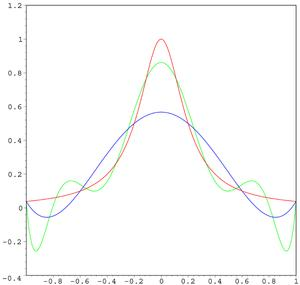
\includegraphics[scale=1]{figures/runge}
  \caption{Runge`s phenomenom}
\end{figure} 

% \newpage
% \bibliographystyle{plain}
% \bibliography{mybib}


\end{document}

